\subsection{Model evaluation and selection} \label{modelRes}
Training was conducted by training several 2D ResNet models, one for each of the datasets, and using a single video as a constant validation set to tune learning rate, weight decay and the dropout layers. For loss functions binary cross entropy was used and for optimization Adam was used. Each model was trained for 65 epochs with a learning rate of $10^{-5}$. No weight decay was added. The true segmentations was 'artificially' constructed by concatenating a vector of zeros equal in length to the number of frames up to the true separation point, and a vector of ones equal in length to the remaining frames of the video, such that we get one continuous block of inflammation predictions followed by one continuous block of healthy predictions which correspond to how the doctor annotated the video.\\ 
In this section two results will be reported. First a five fold approach used to evaluate the model performance where each dataset is split in five folds, then a model is trained on four folds and evaluated on the constant validation set. Second, models are trained on all the data from each dataset respectively, and then used to predict each frame in the validation set for visual inspection.

\begin{table}[H]
	\hspace{-2.2cm}
	\begin{tabular}{|l|cc|cc|cc|cc|cc|r|r|r|}
		\hline
		\multicolumn{1}{|c|}{Dataset}    & \multicolumn{2}{c|}{Fold 1}                                                                                                     & \multicolumn{2}{c|}{Fold 2}                                                                                                     & \multicolumn{2}{c|}{Fold 3}                                                                                                     & \multicolumn{2}{c|}{Fold 4}                                                                                                     & \multicolumn{2}{c|}{Fold 5}                                                                                                     & \multicolumn{1}{c|}{Avg. T}           & \multicolumn{1}{c|}{Avg. V}           & \multicolumn{1}{c|}{Frames} \\ \hline
		\multicolumn{1}{|c|}{}           & \multicolumn{1}{c|}{T}                                                    & V                                                   & \multicolumn{1}{c|}{T}                                                    & V                                                   & \multicolumn{1}{c|}{T}                                                    & V                                                   & \multicolumn{1}{c|}{T}                                                    & V                                                   & \multicolumn{1}{c|}{T}                                                    & V                                                   & \multicolumn{1}{l|}{}                 & \multicolumn{1}{l|}{}                 & \multicolumn{1}{l|}{}       \\ \hline
		Idx\_4\_skip\_10                 & \multicolumn{1}{c|}{\cellcolor[HTML]{FFC7CE}{\color[HTML]{9C0006} 100.0}} & \cellcolor[HTML]{C6EFCE}{\color[HTML]{006100} 67.9} & \multicolumn{1}{c|}{\cellcolor[HTML]{FFC7CE}{\color[HTML]{9C0006} 100.0}} & \cellcolor[HTML]{C6EFCE}{\color[HTML]{006100} 33.2} & \multicolumn{1}{c|}{\cellcolor[HTML]{FFC7CE}{\color[HTML]{9C0006} 100.0}} & \cellcolor[HTML]{C6EFCE}{\color[HTML]{006100} 35.5} & \multicolumn{1}{c|}{\cellcolor[HTML]{FFC7CE}{\color[HTML]{9C0006} 100.0}} & \cellcolor[HTML]{C6EFCE}{\color[HTML]{006100} 43.1} & \multicolumn{1}{c|}{\cellcolor[HTML]{FFC7CE}{\color[HTML]{9C0006} 100.0}} & \cellcolor[HTML]{C6EFCE}{\color[HTML]{006100} 45.9} & {\color[HTML]{7F7F7F} \textit{100}}   & {\color[HTML]{7F7F7F} \textit{45.12}} & 499                         \\ \hline
		Idx\_4\_5\_skip\_20              & \multicolumn{1}{c|}{\cellcolor[HTML]{FFC7CE}{\color[HTML]{9C0006} 99.2}}  & \cellcolor[HTML]{C6EFCE}{\color[HTML]{006100} 47.2} & \multicolumn{1}{c|}{\cellcolor[HTML]{FFC7CE}{\color[HTML]{9C0006} 100.0}} & \cellcolor[HTML]{C6EFCE}{\color[HTML]{006100} 41.0} & \multicolumn{1}{c|}{\cellcolor[HTML]{FFC7CE}{\color[HTML]{9C0006} 99.8}}  & \cellcolor[HTML]{C6EFCE}{\color[HTML]{006100} 35.6} & \multicolumn{1}{c|}{\cellcolor[HTML]{FFC7CE}{\color[HTML]{9C0006} 100.0}} & \cellcolor[HTML]{C6EFCE}{\color[HTML]{006100} 39.0} & \multicolumn{1}{c|}{\cellcolor[HTML]{FFC7CE}{\color[HTML]{9C0006} 99.5}}  & \cellcolor[HTML]{C6EFCE}{\color[HTML]{006100} 33.0} & {\color[HTML]{7F7F7F} \textit{99.7}}  & {\color[HTML]{7F7F7F} \textit{39.16}} & 500                         \\ \hline
		Idx\_2\_3\_4\_5\_6\_skip\_50     & \multicolumn{1}{c|}{\cellcolor[HTML]{FFC7CE}{\color[HTML]{9C0006} 99.5}}  & \cellcolor[HTML]{C6EFCE}{\color[HTML]{006100} 71.4} & \multicolumn{1}{c|}{\cellcolor[HTML]{FFC7CE}{\color[HTML]{9C0006} 99.5}}  & \cellcolor[HTML]{C6EFCE}{\color[HTML]{006100} 63.7} & \multicolumn{1}{c|}{\cellcolor[HTML]{FFC7CE}{\color[HTML]{9C0006} 99.5}}  & \cellcolor[HTML]{C6EFCE}{\color[HTML]{006100} 70.0} & \multicolumn{1}{c|}{\cellcolor[HTML]{FFC7CE}{\color[HTML]{9C0006} 99.7}}  & \cellcolor[HTML]{C6EFCE}{\color[HTML]{006100} 45.5} & \multicolumn{1}{c|}{\cellcolor[HTML]{FFC7CE}{\color[HTML]{9C0006} 100.0}} & \cellcolor[HTML]{C6EFCE}{\color[HTML]{006100} 43.4} & {\color[HTML]{7F7F7F} \textit{99.64}} & {\color[HTML]{7F7F7F} \textit{58.8}}  & 491                         \\ \hline
		Idx\_2\_3\_4\_5\_6\_skip\_20     & \multicolumn{1}{c|}{\cellcolor[HTML]{FFC7CE}{\color[HTML]{9C0006} 100.0}} & \cellcolor[HTML]{C6EFCE}{\color[HTML]{006100} 60.9} & \multicolumn{1}{c|}{\cellcolor[HTML]{FFC7CE}{\color[HTML]{9C0006} 99.7}}  & \cellcolor[HTML]{C6EFCE}{\color[HTML]{006100} 61.8} & \multicolumn{1}{c|}{\cellcolor[HTML]{FFC7CE}{\color[HTML]{9C0006} 99.7}}  & \cellcolor[HTML]{C6EFCE}{\color[HTML]{006100} 66.2} & \multicolumn{1}{c|}{\cellcolor[HTML]{FFC7CE}{\color[HTML]{9C0006} 99.7}}  & \cellcolor[HTML]{C6EFCE}{\color[HTML]{006100} 71.4} & \multicolumn{1}{c|}{\cellcolor[HTML]{FFC7CE}{\color[HTML]{9C0006} 99.8}}  & \cellcolor[HTML]{C6EFCE}{\color[HTML]{006100} 65.5} & {\color[HTML]{7F7F7F} \textit{99.78}} & {\color[HTML]{7F7F7F} \textit{65.16}} & 1226                        \\ \hline
		Idx\_4\_14\_18\_20\_32\_skip\_20 & \multicolumn{1}{c|}{\cellcolor[HTML]{FFC7CE}{\color[HTML]{9C0006} 99.7}}  & \cellcolor[HTML]{C6EFCE}{\color[HTML]{006100} 33.9} & \multicolumn{1}{c|}{\cellcolor[HTML]{FFC7CE}{\color[HTML]{9C0006} 100.0}} & \cellcolor[HTML]{C6EFCE}{\color[HTML]{006100} 42.6} & \multicolumn{1}{c|}{\cellcolor[HTML]{FFC7CE}{\color[HTML]{9C0006} 99.9}}  & \cellcolor[HTML]{C6EFCE}{\color[HTML]{006100} 40.6} & \multicolumn{1}{c|}{\cellcolor[HTML]{FFC7CE}{\color[HTML]{9C0006} 99.9}}  & \cellcolor[HTML]{C6EFCE}{\color[HTML]{006100} 37.2} & \multicolumn{1}{c|}{\cellcolor[HTML]{FFC7CE}{\color[HTML]{9C0006} 99.8}}  & \cellcolor[HTML]{C6EFCE}{\color[HTML]{006100} 38.2} & {\color[HTML]{7F7F7F} \textit{99.86}} & {\color[HTML]{7F7F7F} \textit{38.5}}  & 997                         \\ \hline
		Idx\_4\_14\_18\_20\_32\_skip\_5  & \multicolumn{1}{c|}{\cellcolor[HTML]{FFC7CE}{\color[HTML]{9C0006} 99.9}}  & \cellcolor[HTML]{C6EFCE}{\color[HTML]{006100} 69.3} & \multicolumn{1}{c|}{\cellcolor[HTML]{FFC7CE}{\color[HTML]{9C0006} 100.0}} & \cellcolor[HTML]{C6EFCE}{\color[HTML]{006100} 57.1} & \multicolumn{1}{c|}{\cellcolor[HTML]{FFC7CE}{\color[HTML]{9C0006} 86.4}}  & \cellcolor[HTML]{C6EFCE}{\color[HTML]{006100} 39.5} & \multicolumn{1}{c|}{\cellcolor[HTML]{FFC7CE}{\color[HTML]{9C0006} 99.5}}  & \cellcolor[HTML]{C6EFCE}{\color[HTML]{006100} 55.9} & \multicolumn{1}{c|}{\cellcolor[HTML]{FFC7CE}{\color[HTML]{9C0006} 99.9}}  & \cellcolor[HTML]{C6EFCE}{\color[HTML]{006100} 60.9} & {\color[HTML]{7F7F7F} \textit{97.14}} & {\color[HTML]{7F7F7F} \textit{56.54}} & 3978                        \\ \hline
		Idx\_3\_23\_skip\_10             & \multicolumn{1}{c|}{\cellcolor[HTML]{FFC7CE}{\color[HTML]{9C0006} 100.0}} & \cellcolor[HTML]{C6EFCE}{\color[HTML]{006100} 72.0} & \multicolumn{1}{c|}{\cellcolor[HTML]{FFC7CE}{\color[HTML]{9C0006} 100.0}} & \cellcolor[HTML]{C6EFCE}{\color[HTML]{006100} 72.3} & \multicolumn{1}{c|}{\cellcolor[HTML]{FFC7CE}{\color[HTML]{9C0006} 100.0}} & \cellcolor[HTML]{C6EFCE}{\color[HTML]{006100} 72.6} & \multicolumn{1}{c|}{\cellcolor[HTML]{FFC7CE}{\color[HTML]{9C0006} 100.0}} & \cellcolor[HTML]{C6EFCE}{\color[HTML]{006100} 72.4} & \multicolumn{1}{c|}{\cellcolor[HTML]{FFC7CE}{\color[HTML]{9C0006} 100.0}} & \cellcolor[HTML]{C6EFCE}{\color[HTML]{006100} 70.6} & {\color[HTML]{7F7F7F} \textit{100.0}} & {\color[HTML]{7F7F7F} \textit{72.0}}  & 829                         \\ \hline
		Idx\_19\_24\_skip\_5             & \multicolumn{1}{c|}{\cellcolor[HTML]{FFC7CE}{\color[HTML]{9C0006} 100.0}} & \cellcolor[HTML]{C6EFCE}{\color[HTML]{006100} 26.8} & \multicolumn{1}{c|}{\cellcolor[HTML]{FFC7CE}{\color[HTML]{9C0006} 100.0}} & \cellcolor[HTML]{C6EFCE}{\color[HTML]{006100} 25.9} & \multicolumn{1}{c|}{\cellcolor[HTML]{FFC7CE}{\color[HTML]{9C0006} 99.8}}  & \cellcolor[HTML]{C6EFCE}{\color[HTML]{006100} 27.7} & \multicolumn{1}{c|}{\cellcolor[HTML]{FFC7CE}{\color[HTML]{9C0006} 100.0}} & \cellcolor[HTML]{C6EFCE}{\color[HTML]{006100} 27.3} & \multicolumn{1}{c|}{\cellcolor[HTML]{FFC7CE}{\color[HTML]{9C0006} 100.0}} & \cellcolor[HTML]{C6EFCE}{\color[HTML]{006100} 26.7} & {\color[HTML]{7F7F7F} \textit{100.0}} & {\color[HTML]{7F7F7F} \textit{26.9}}  & 600                         \\ \hline
	\end{tabular}
	\caption{Evaluation results for training a modified 2D ResNet on different datasets. All results are in percent. At each fold, T stands for training accuracy and V stands for validation accuracy.}
	\label{2dresnetevalres}
\end{table}

In \autoref{2dresnetevalres} we see the evaluation of the five fold approach. T stands for training accuracy and V stands for validation accuracy. All results are reported in percent. We note dataset \textit{Idx\_3\_23\_skip\_10} and \textit{Idx\_2\_3\_4\_5\_6\_skip\_20} have the highest validation accuracies while \textit{Idx\_19\_24\_skip\_5} has the lowest followed by \textit{Idx\_4\_14\_18\_20\_32\_} \textit{skip\_5}. We also note there seemingly is no relation between the sheer number of training images and high validation accuracy, but there is some relation when we chose to add more images from the same dataset. Likewise there is seemingly no relation between the different number of patients the training images comes from and high validation accuracy.

To assert whether the reported accuracies are accurate, we will now take a look at how the models predicted on some videos. First we will look at how each of the models predicted on the validation video to establish a baseline. The results can be seen in \autoref{firstfive} and in \autoref{lastthree}. For each illustration the true segmentation of the video has been drawn as the first bar. For these results, this means approximately 72\% of the frames are annotated as inflamed and the last frames as healthy. The second bar is the model predictions. The blue line indicates the models' confidence in a healthy prediction, and a probability above 50\% means it has predicted the frame is healthy.

\begin{figure}[H]
	\centering
	\begin{subfigure}{\linewidth}
		\centering
		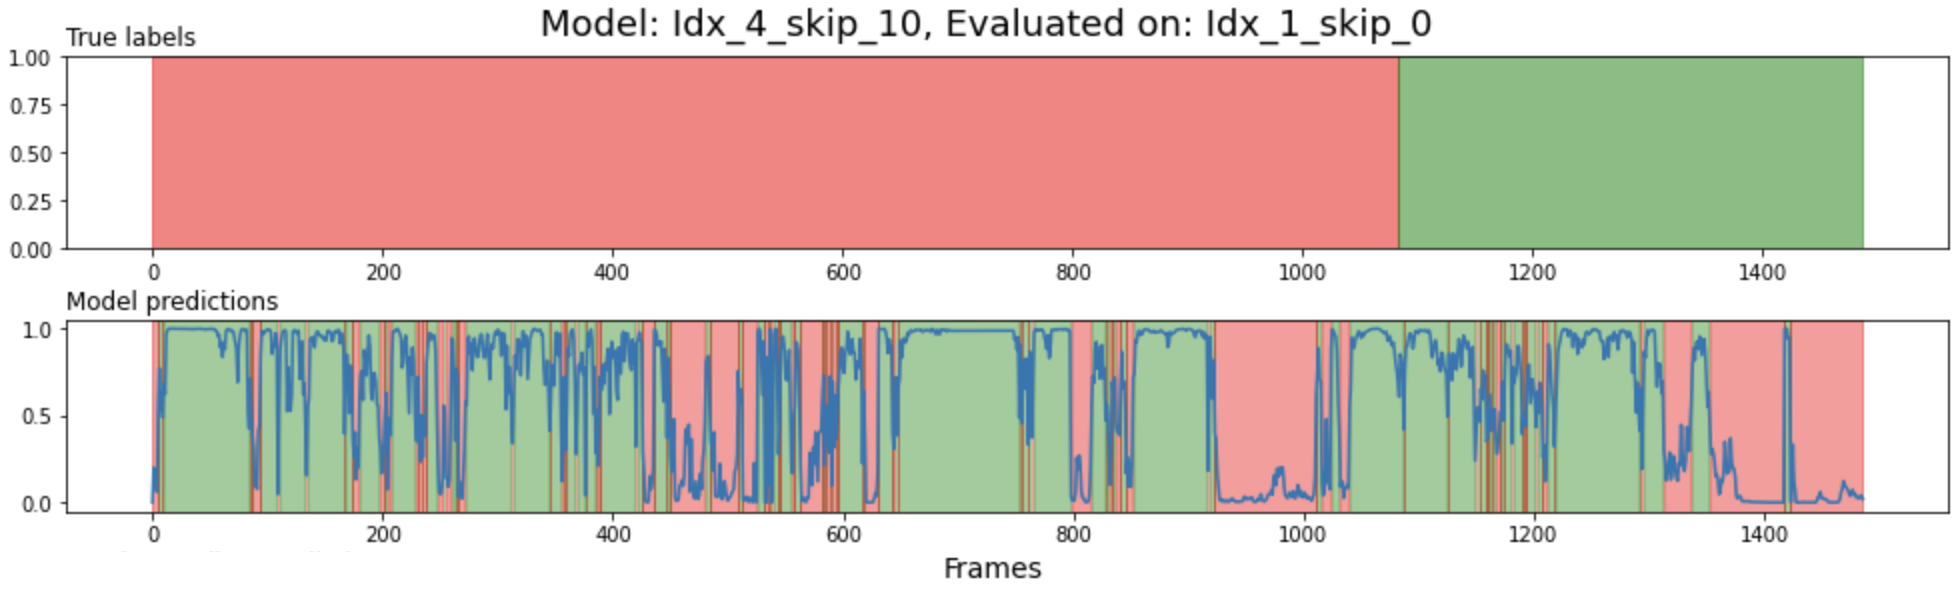
\includegraphics[width=\linewidth]{Materials/Results/SP/M1On1C}
	\end{subfigure}
	\\
	\begin{subfigure}{\linewidth}
		\centering
		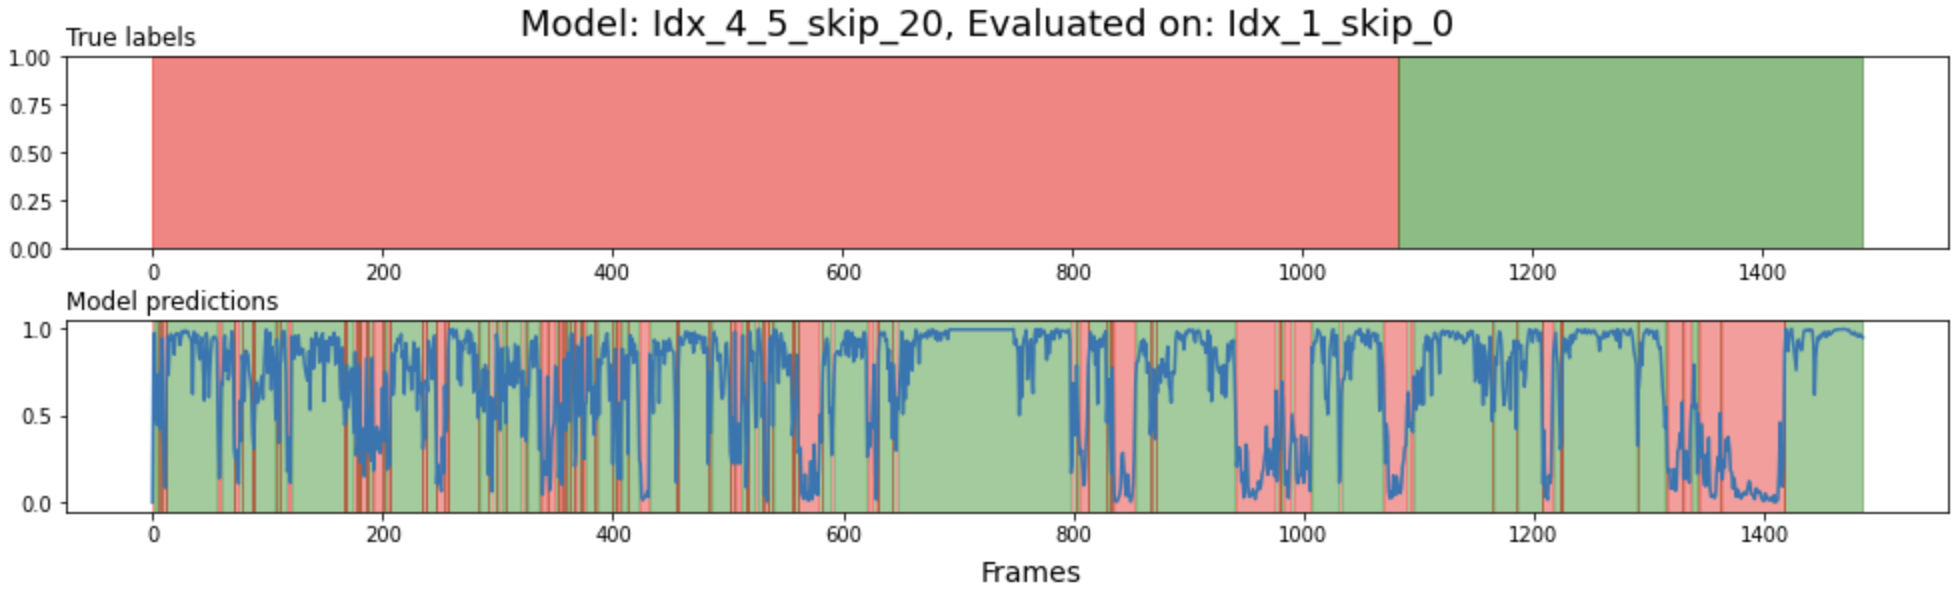
\includegraphics[width=\linewidth]{Materials/Results/SP/M2On1C}
	\end{subfigure}
	\\
	\begin{subfigure}{\linewidth}
		\centering
		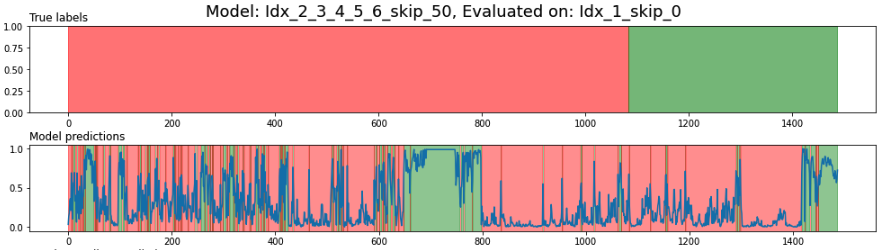
\includegraphics[width=\linewidth]{Materials/Results/SP/M3On1C}
	\end{subfigure}
	\\
	\begin{subfigure}{\linewidth}
		\centering
		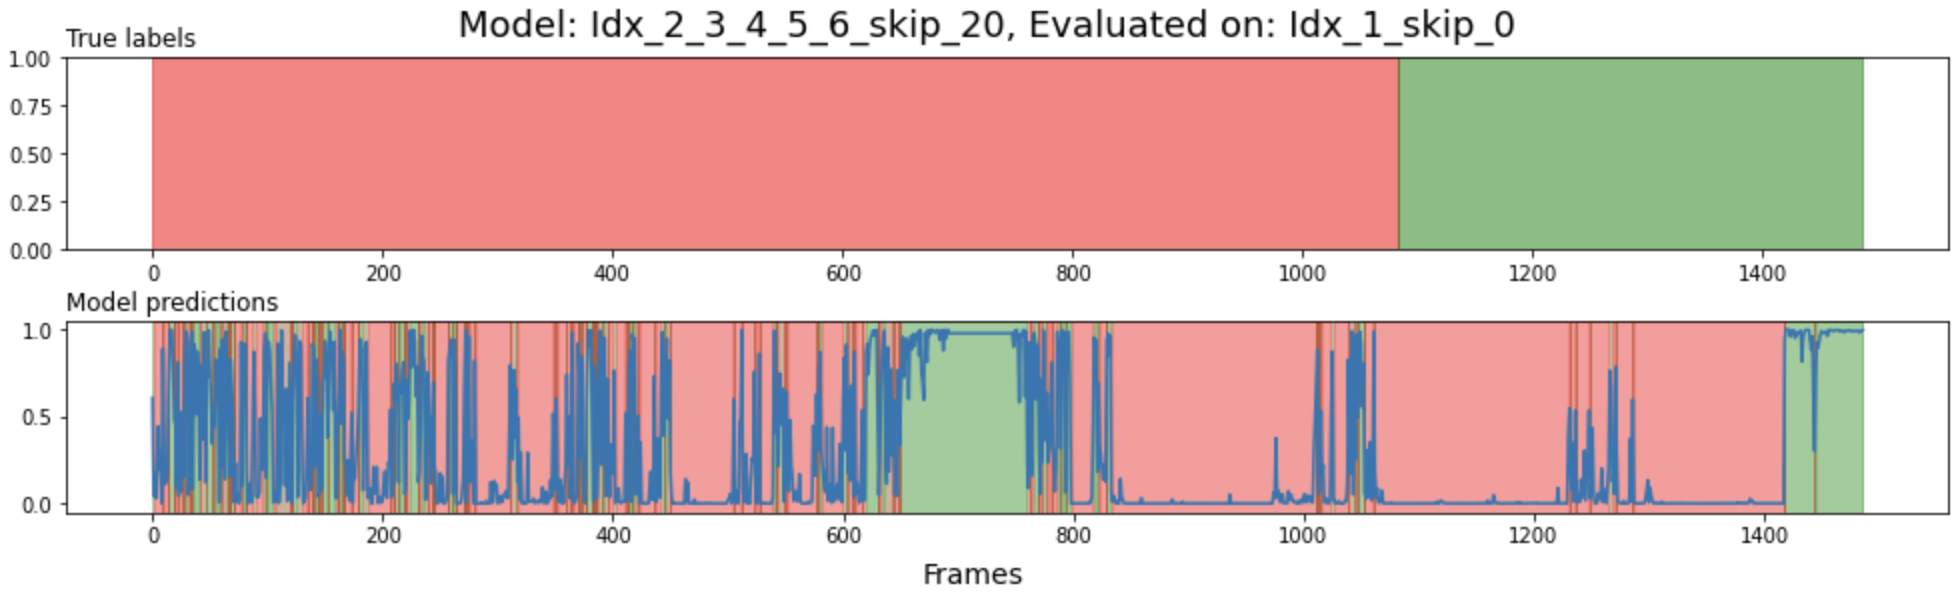
\includegraphics[width=\linewidth]{Materials/Results/SP/M4On1C}
	\end{subfigure}
	\\
	\begin{subfigure}{\linewidth}
		\centering
		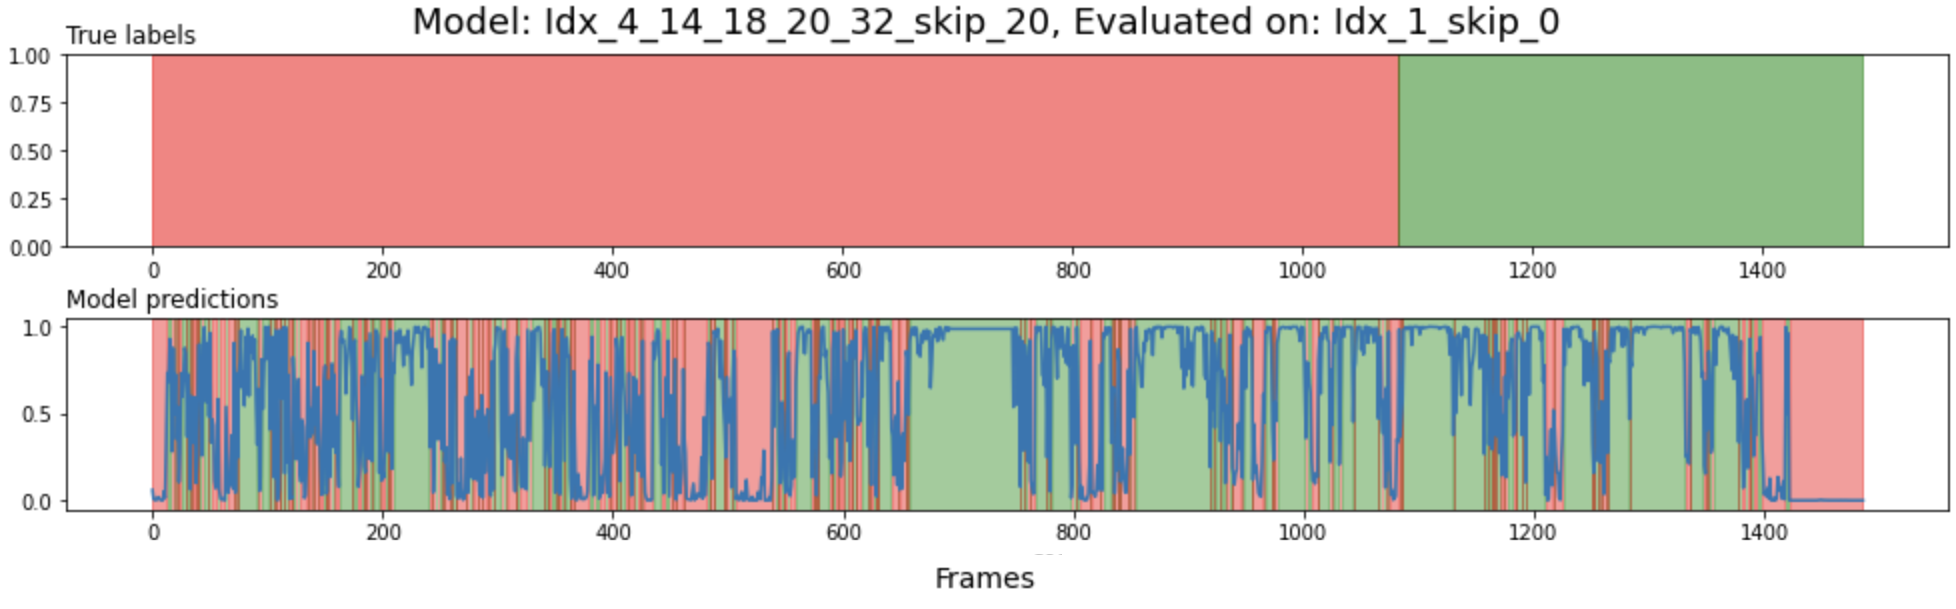
\includegraphics[width=\linewidth]{Materials/Results/SP/M5On1C}
	\end{subfigure}
	\caption{How the first five models predicted on the validation video.}
	\label{firstfive}
\end{figure}

\begin{figure}[H]
	\centering
	\begin{subfigure}{\linewidth}
		\centering
		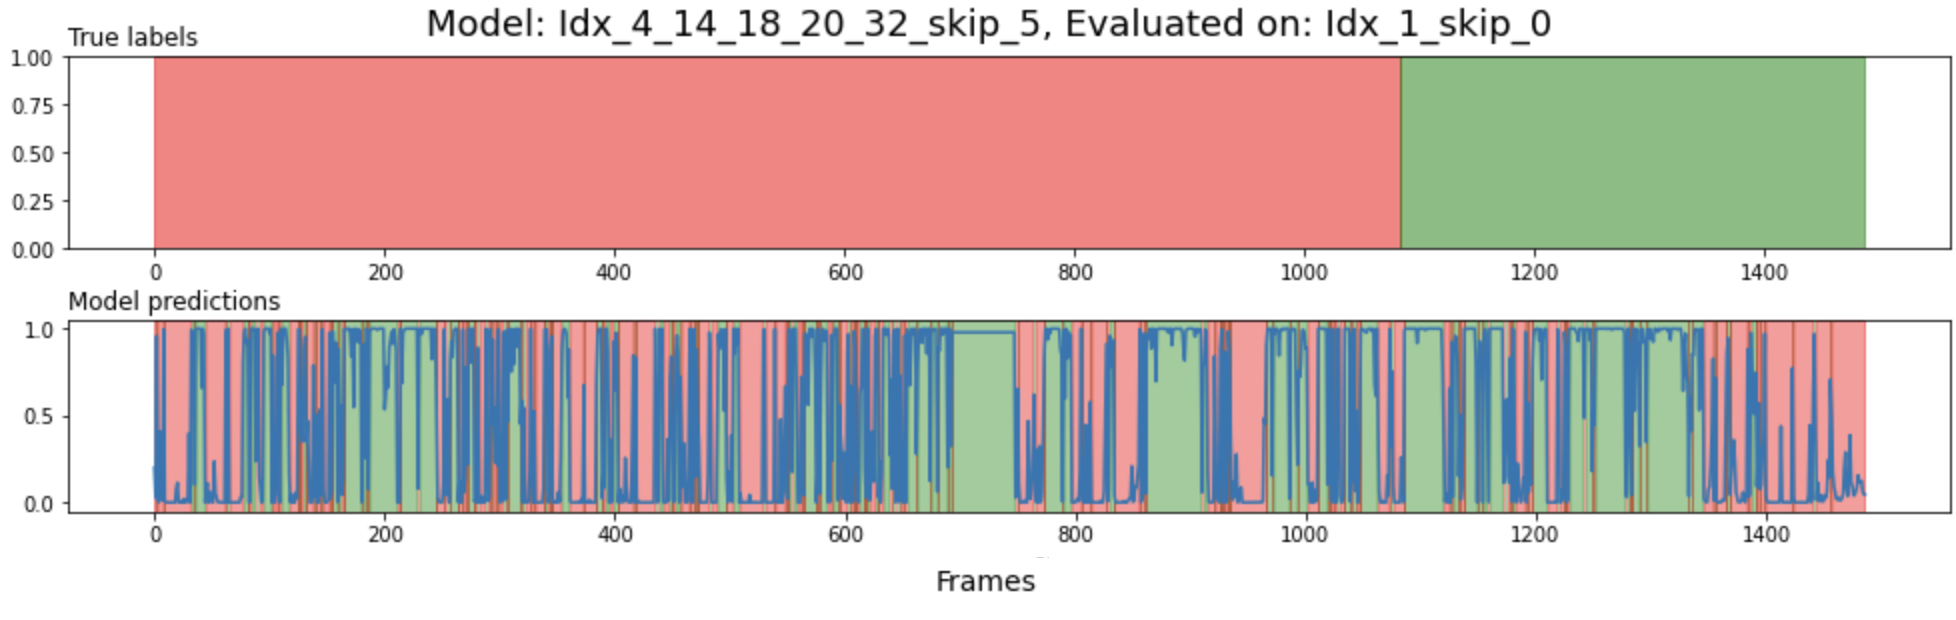
\includegraphics[width=\linewidth]{Materials/Results/SP/M6On1C}
	\end{subfigure}
	\\
	\begin{subfigure}{\linewidth}
		\centering
		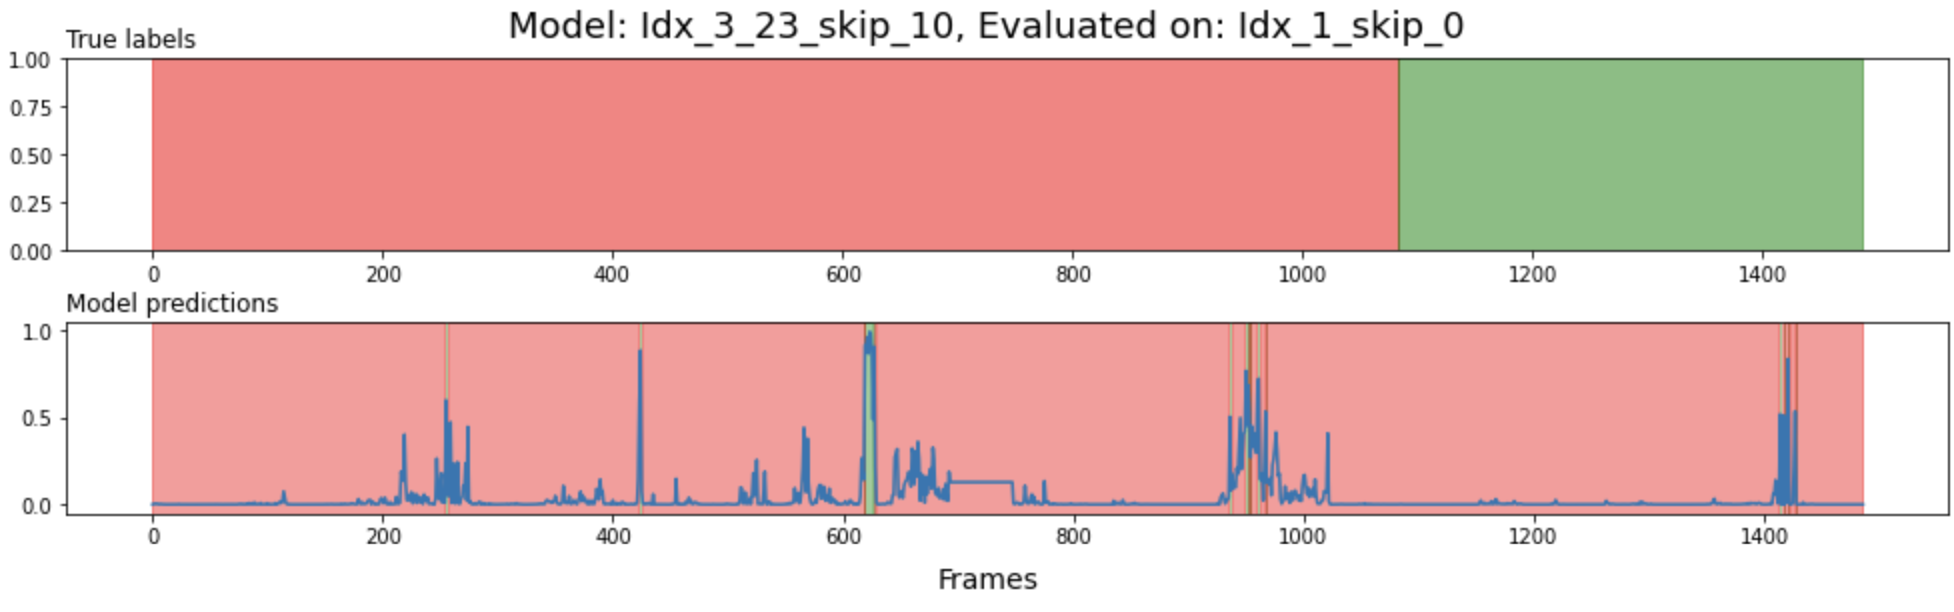
\includegraphics[width=\linewidth]{Materials/Results/SP/M7On1C}
	\end{subfigure}
	\\
	\begin{subfigure}{\linewidth}
		\centering
		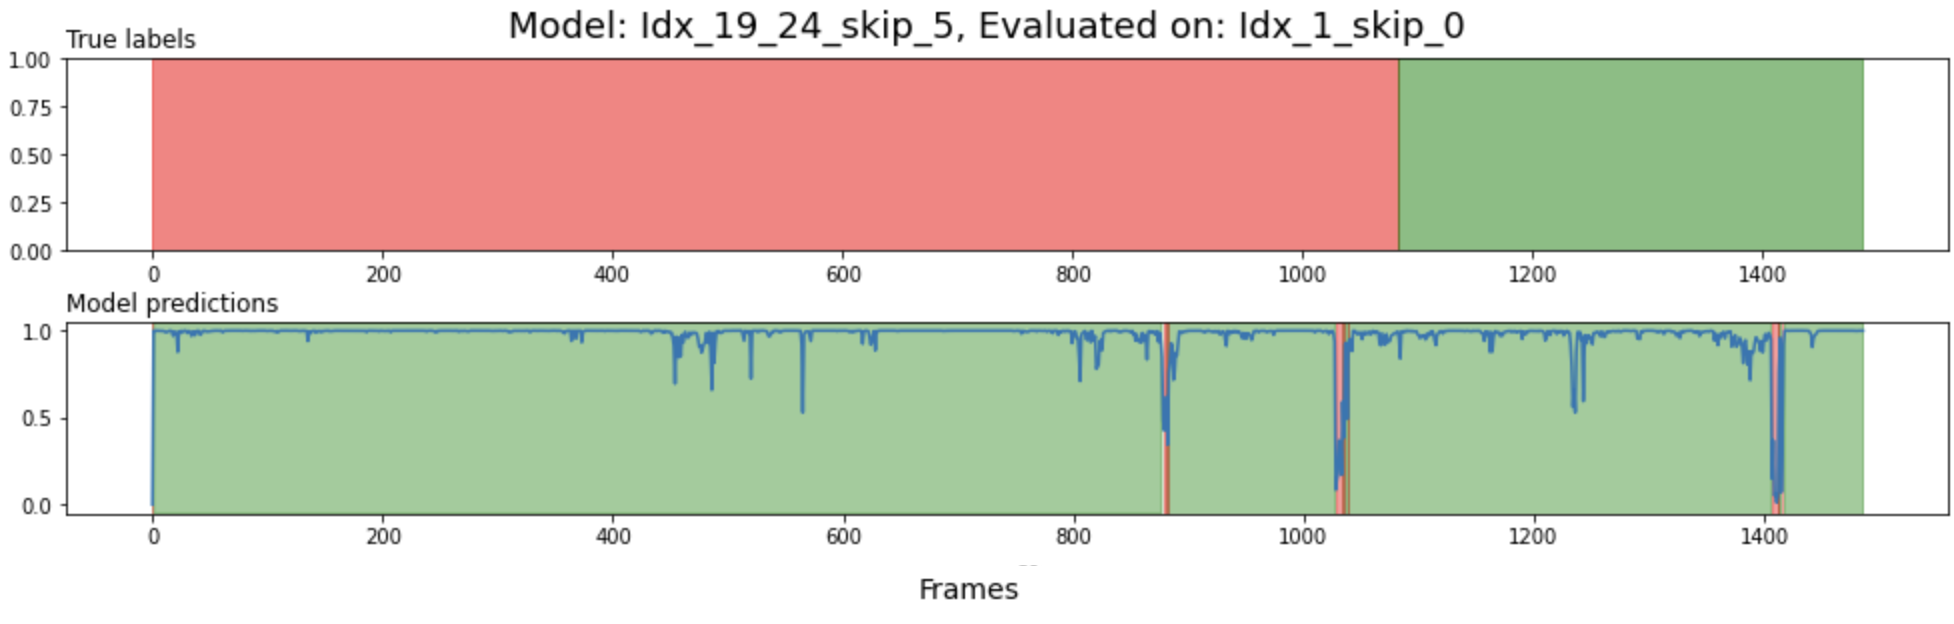
\includegraphics[width=\linewidth]{Materials/Results/SP/M8On1C}
	\end{subfigure}
	\caption{How the last three models predicted on the validation video.}
	\label{lastthree}
\end{figure}

We note how models \textit{Idx\_4\_skip\_10} and \textit{Idx\_4\_5\_skip\_20} predict overly many healthy frames but seem to be fairly confident in their predictions. Model \textit{Idx\_2\_3\_4\_5\_6\_skip\_50} have comparably predicted a lot more inflamed frames, but it still seem to be confident some of the first frames are healthy. Looking at model \textit{Idx\_2\_3\_4\_5\_6\_skip\_20} which scored the second highest validation accuracy, we see it has some rather volatile predictions on the early frames where most however seem to be classified as inflamed. On the other hand, it seem to predict quite confidently too many inflamed frames towards the end of the video. Model \textit{Idx\_4\_14\_18\_20\_32\_skip\_20} is the first model trained across several patients, but this models seem to predict a mix of the previous models as it has some volatile predictions in the beginning of the video, but towards the middle it begins to confidently predict overly many healthy frames. Model \textit{Idx\_4\_14\_18\_20\_32\_skip\_5} is the second model to be trained on several patients and also had a significant larger training set than the other models. Here we see only a few blocks of consecutive healthy predictions and otherwise some very volatile predictions. Towards the end of the video it predicts a large part correctly healthy, but it also predicts the very end inflamed. Model \textit{Idx\_3\_23\_skip\_10} was the model which achieved the highest validation accuracies, but we also see it very rarely predicts other than inflamed. As the validation video

\begin{figure}[H]
	\centering
	\begin{subfigure}{\linewidth}
		\centering
		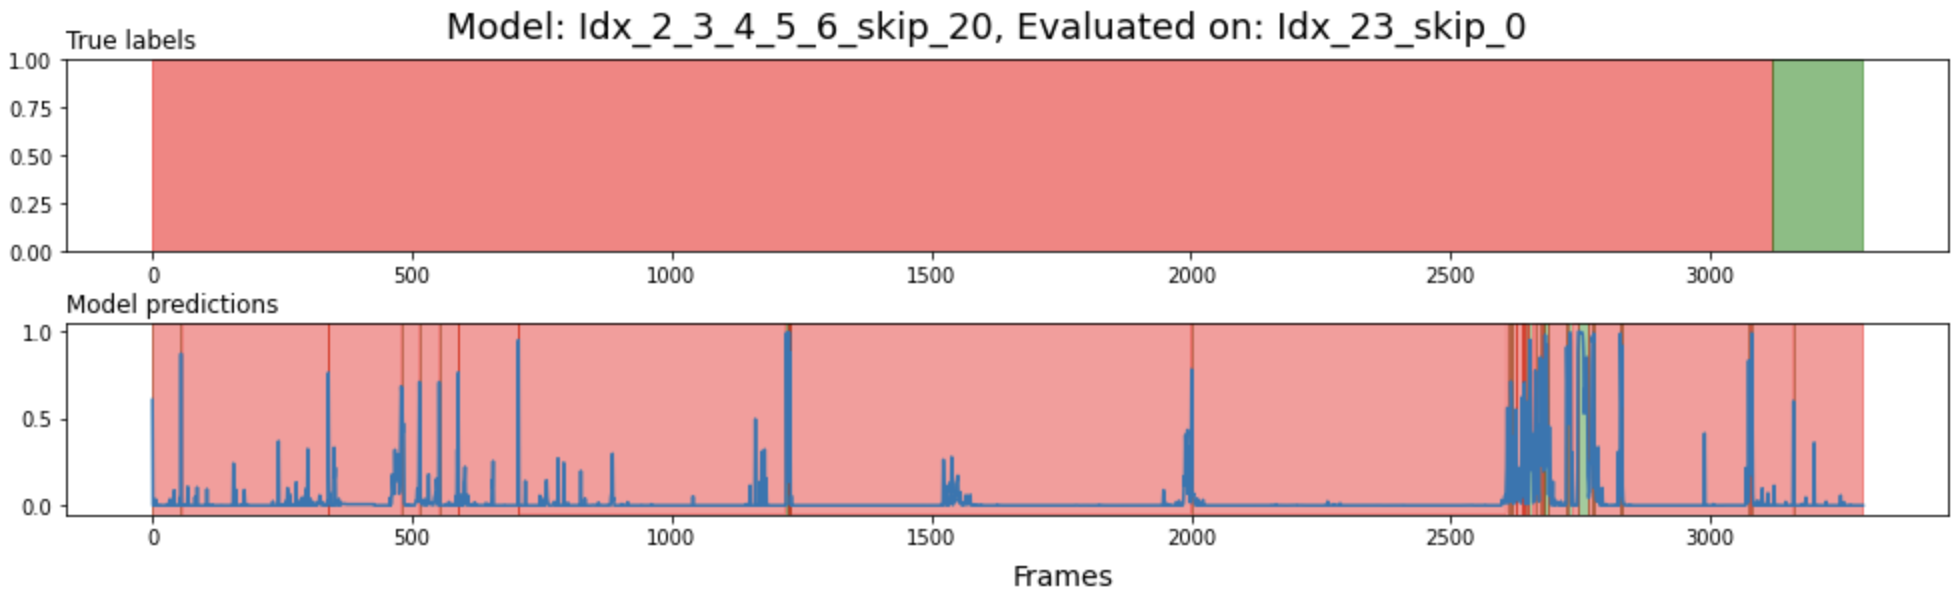
\includegraphics[width=\linewidth]{Materials/Results/SP/M4On23C}
	\end{subfigure}
	\\
	\begin{subfigure}{\linewidth}
		\centering
		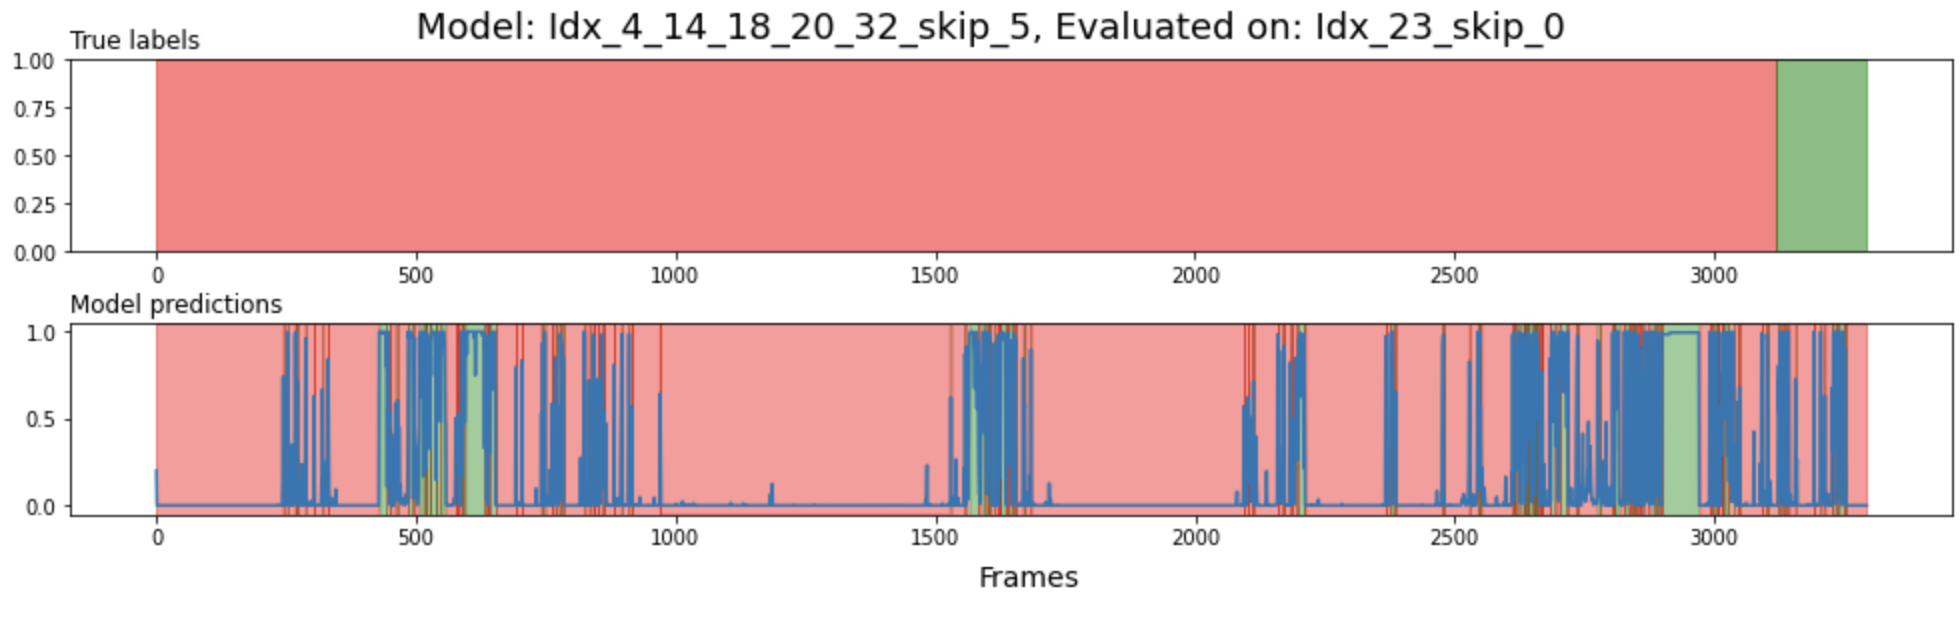
\includegraphics[width=\linewidth]{Materials/Results/SP/M6On23C}
	\end{subfigure}
	\caption{How the two selected models perform on test set \textit{Idx\_23\_skip\_0}.}
	\label{idx23}
\end{figure}

consists of approximately 72\% inflamed frames, it would seem its accuracy is skewed because of the imbalance in the data. Lastly we have model \textit{Idx\_19\_24\_skip\_5} which has the opposite issue where it only predicts healthy.

To select which model to move forward and perform treatment predictions with, models \textit{Idx\_2\_3\_4\_5\_6\_skip\_20} and \textit{Idx\_4\_14\_18\_20\_32\_skip\_5} were selected to predict on more videos. \textit{Idx\_2\_3\_4\_5\_6\_skip\_20} was selected as it seem to predict the best on the validation video and \textit{Idx\_4\_14\_18\_20\_32\_skip\_5} because prior knowledge say models trained on more and varied data should perform better, and thus we verify its validation results from \autoref{2dresnetevalres} are not amiss.

In \autoref{idx23} we see the predictions of the two models on an unseen video which is biased towards being inflamed. We see model \textit{Idx\_2\_3\_4\_5\_6\_skip\_20} predicting confidently and almost exclusively inflammation with a few healthy predictions in the wrong places. Model \textit{Idx\_4\_14\_18\_20\_32\_skip\_5} is more uncertain, and predicts healthy in some spots while having oscillating predictions. The largest consecutive part where it confidently predicts healthy is when it should have predicted inflammation.

In \autoref{idx24} we see the predictions of the two selected models on an unseen video biased towards being healthy. We see model \textit{Idx\_2\_3\_4\_5\_6\_skip\_20} still confidently predicting most frames inflamed, with a few correct exceptions towards the middle of the video. Model \textit{Idx\_4\_14\_18\_20\_32\_skip\_5} predicts most of the video inflamed too, but is not as certain and also correctly predicts one large block healthy.

As a last validation, in \autoref{idx28} we see the predictions of the two selected models on an unseen video biased towards inflammation. Model \textit{Idx\_2\_3\_4\_5\_6\_skip\_20} is rather volatile in its predictions at the beginning of the video, but seem to correctly predict mostly inflammation. Towards the end it seem to capture some of the healthy frames, but predicts a few too many. Model \textit{Idx\_4\_14\_18\_20\_32\_skip\_5} seems on the other hand very volatile, and seem to have some passages where it wrongly predicts healthy. Towards the end we still see some volatile predictions, but it does not seem to capture the healthy frames at the end.

\begin{figure}[H]
	\centering
	\begin{subfigure}{\linewidth}
		\centering
		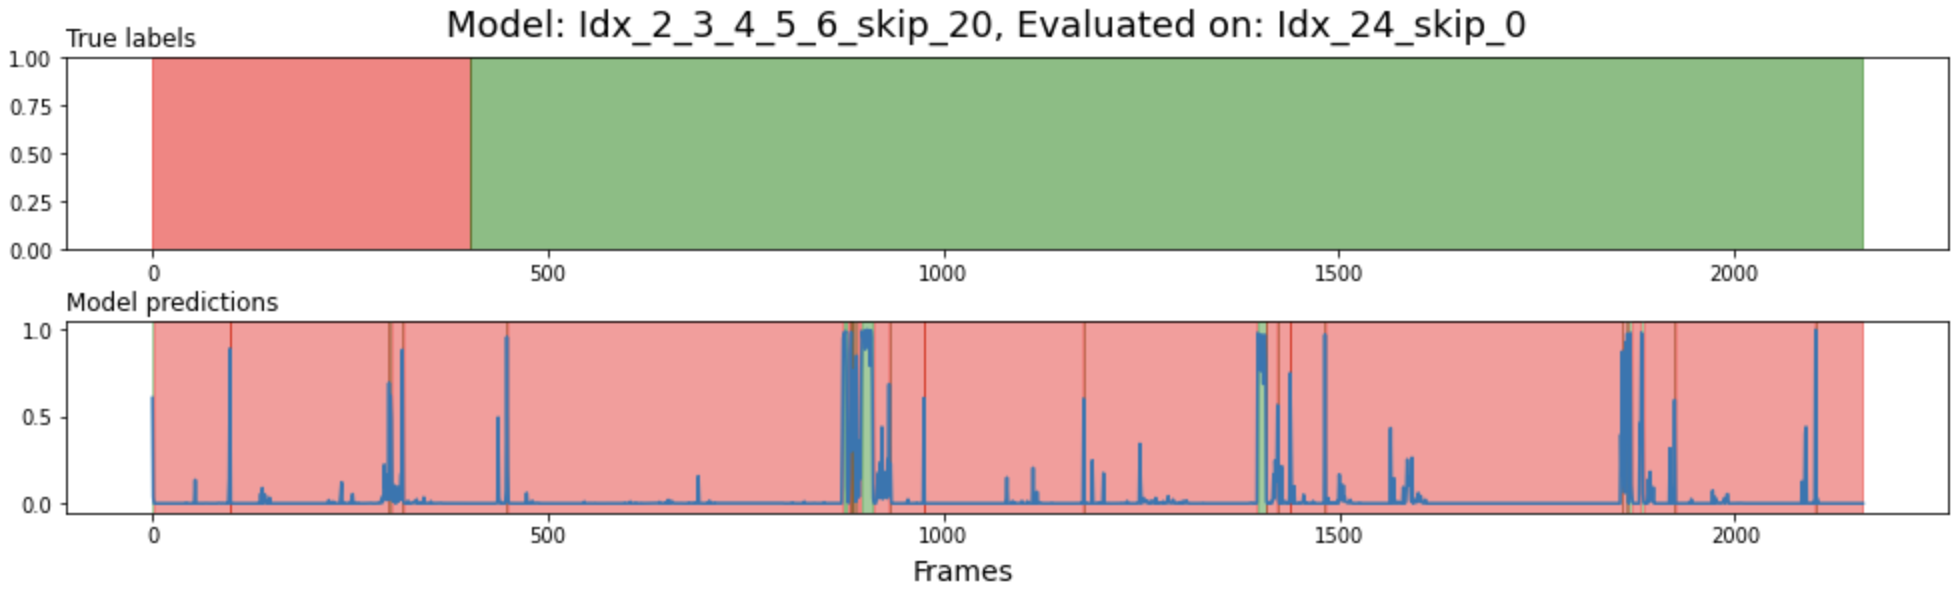
\includegraphics[width=\linewidth]{Materials/Results/SP/M4On24C}
	\end{subfigure}
	\\
	\begin{subfigure}{\linewidth}
		\centering
		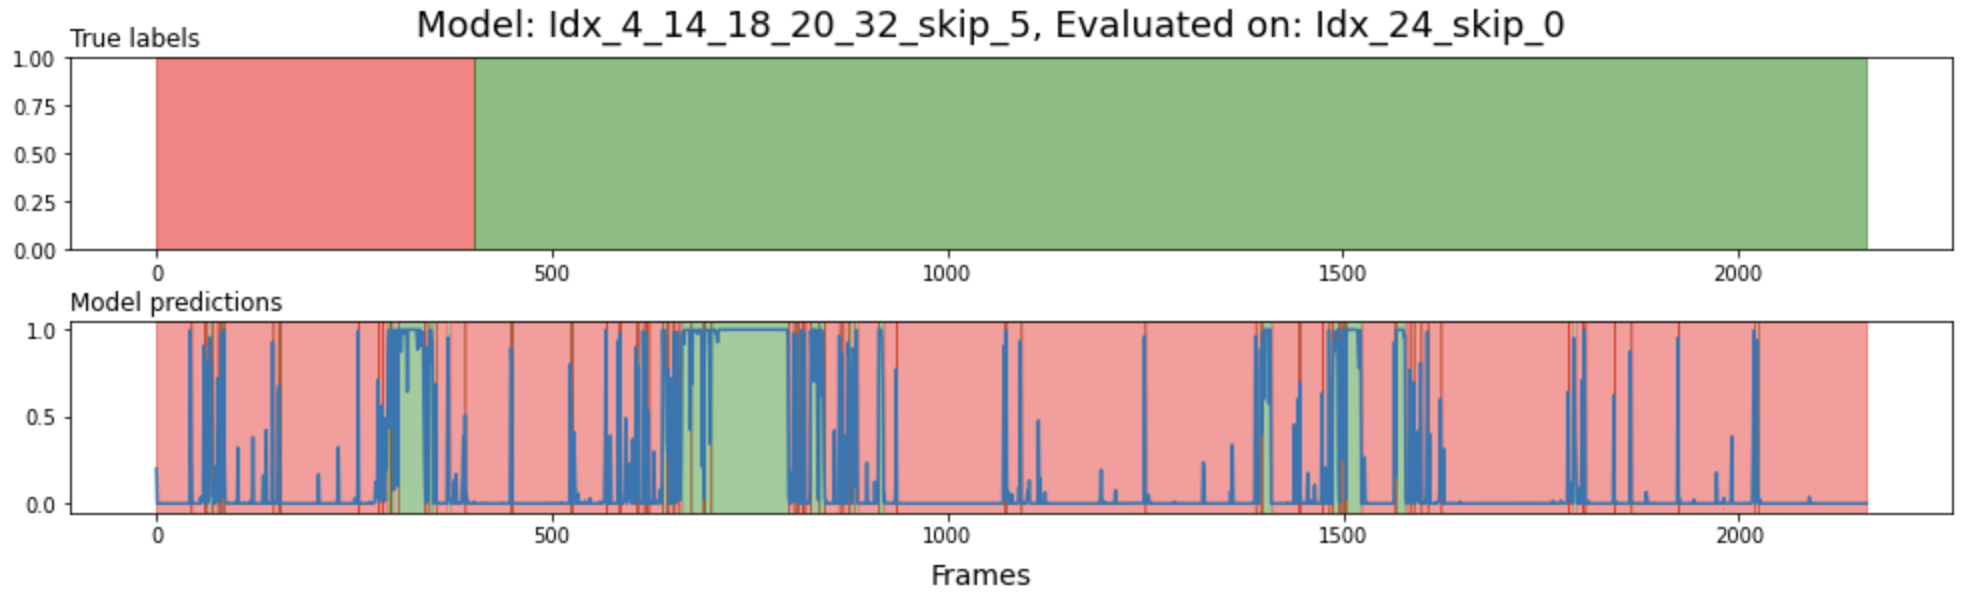
\includegraphics[width=\linewidth]{Materials/Results/SP/M6On24C}
	\end{subfigure}
	\caption{How the two selected models perform on test set \textit{Idx\_24\_skip\_0}.}
	\label{idx24}
\end{figure}

\begin{figure}[H]
	\centering
	\begin{subfigure}{\linewidth}
		\centering
		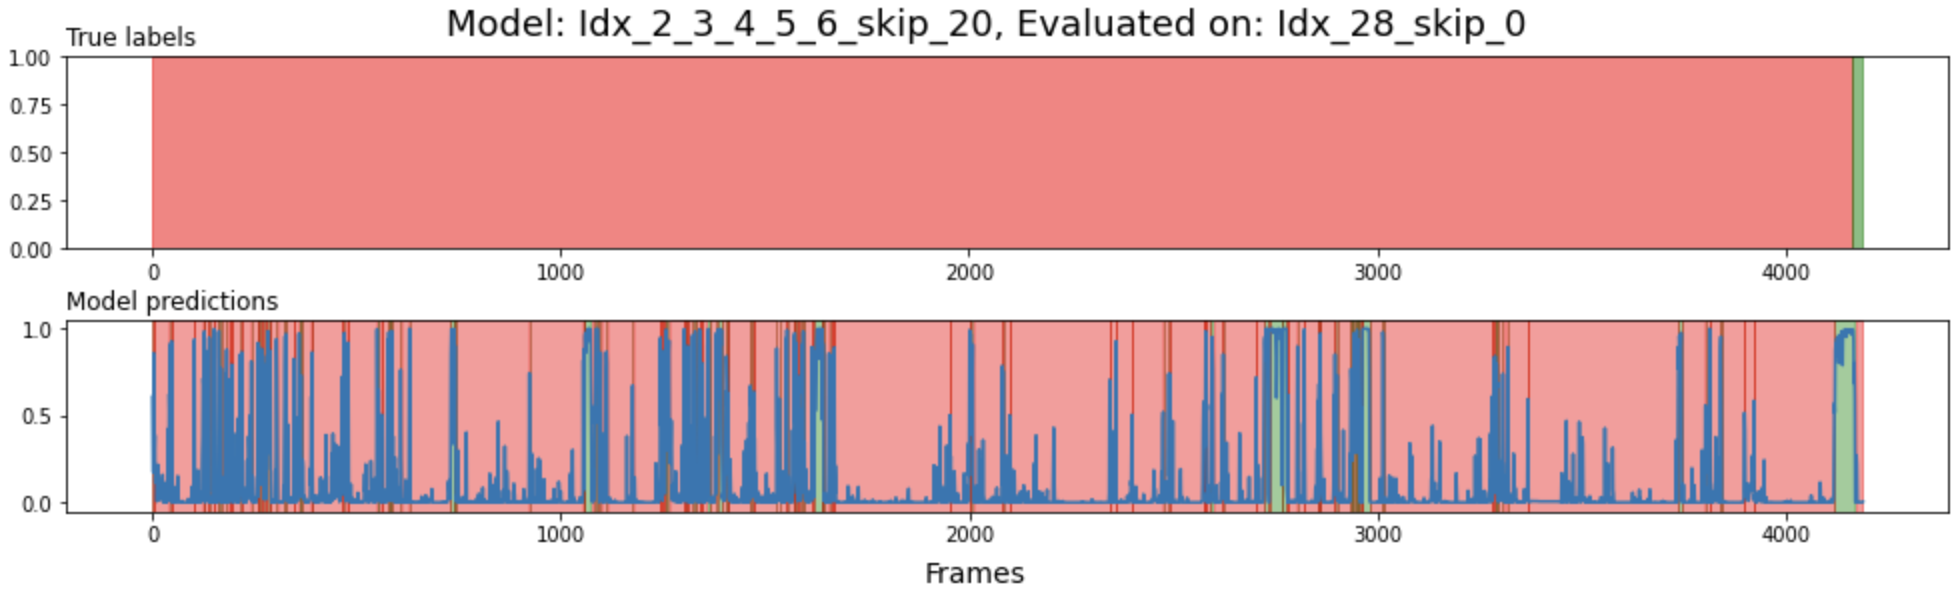
\includegraphics[width=\linewidth]{Materials/Results/SP/M4On28C}
	\end{subfigure}
	\\
	\begin{subfigure}{\linewidth}
		\centering
		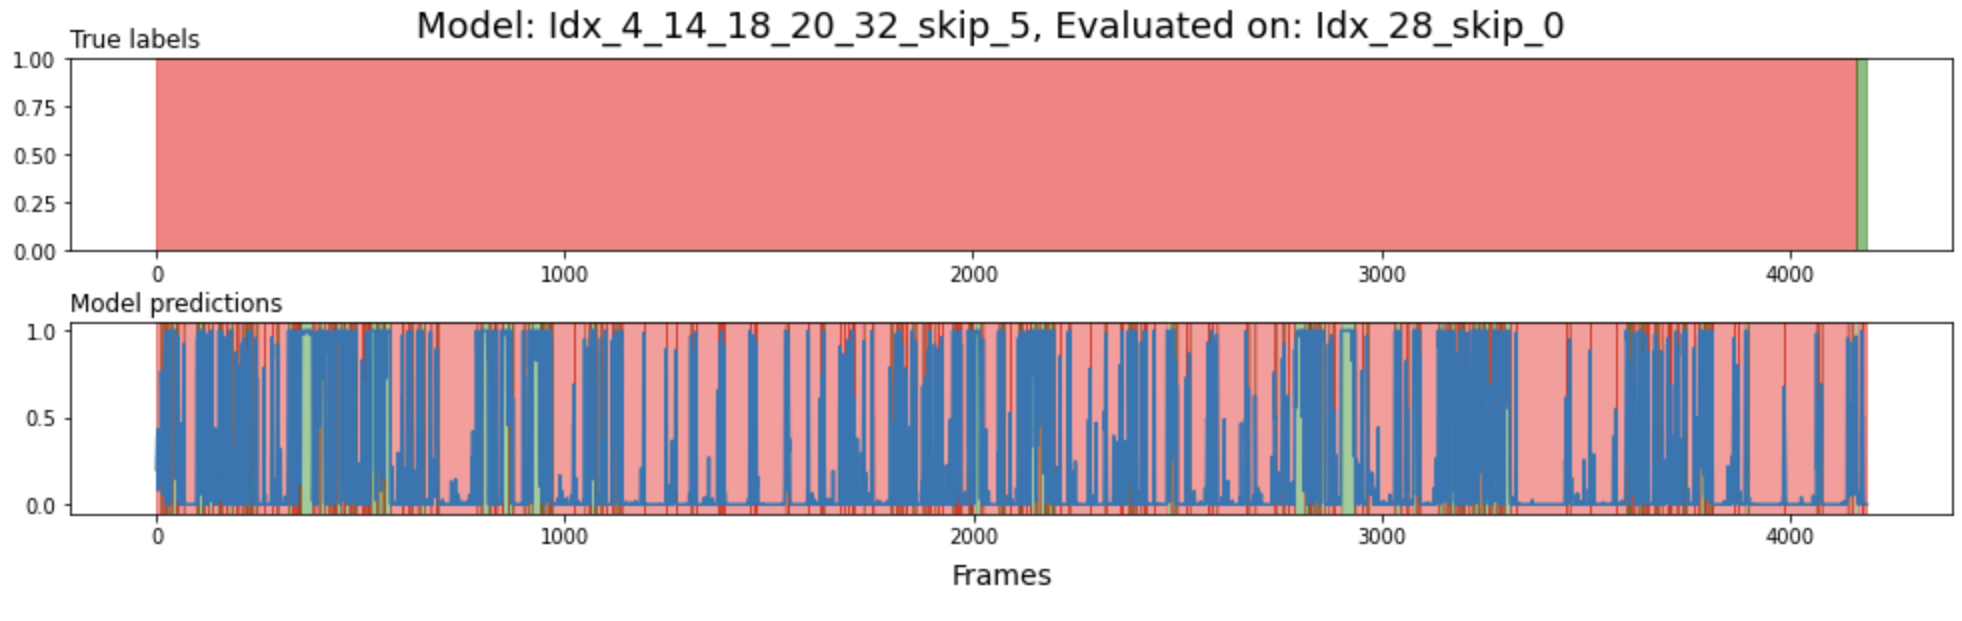
\includegraphics[width=\linewidth]{Materials/Results/SP/M6On28C}
	\end{subfigure}
	\caption{How the two selected models perform on test set \textit{Idx\_28\_skip\_0}.}
	\label{idx28}
\end{figure}

Based on these results model \textit{Idx\_2\_3\_4\_5\_6\_skip\_20} is considered to be the most accurate, and will be used moving forward towards predicting separation points and treatments.